\documentclass{beamer}
\usepackage[T1]{fontenc}
\usepackage[utf8]{inputenc}
\usepackage{lmodern}
\usepackage[brazil]{babel}
\usepackage[labelformat=empty]{caption}
\usepackage{graphicx}
\usetheme{Luebeck}
\title[Padrão Model-View-Controller]{Padrão Model-View-Controller}
\author{Ana Luísa Losnak. Luiz Armesto. Renan Fichberg.}
\date{Novembro 4, 2014}
\institute{Instituto de Matemática e Estatística da Universidade de São Paulo (IME-USP)}
\begin{document}

\begin{frame}
\titlepage
\end{frame}

\begin{frame}
\frametitle{Introdução}
\begin{itemize}
	\item O que é um padrão?
	\item O padrão MVC
	\item Alguns frameworks que usam MVC ou derivados.
	\item Alguns padrões similares ao MVC
\end{itemize}
\end{frame}

%TODO: o que é um padrão (não há necessidade de dar exemplos. O tema por si só já é um exemplo)
\begin{frame}
\frametitle{O que é um padrão?}
	Em Engenharia de Software, um padrão de design é uma solução geral que pode ser reutilizada para resolver um problema recorrente de um contexto específico de Design de Software
\end{frame}

%TODO: O padrão MVC
\begin{frame}
\frametitle{O padrão MVC}
\begin{itemize}
	\item Breve histórico
	\item Por que usar?
	\item O padrão MVC
	\item A tríade: os três componentes do MVC
	\item Padrões associados
\end{itemize}
\end{frame}

\begin{frame}
\frametitle{O padrão MVC}
% Essa explicação é boa para o MVC Model2. No MVC clássico o controller não serve de cola, ele serve para controlar o input.
	`An easy way to understand MVC: the model is the data, the view is the window on the screen, and the controller is the glue between the two.' \\
	\hfill \textit{- Connelly Barnes.}
\end{frame}


\begin{frame}
\frametitle{O padrão MVC}
\framesubtitle{Breve histórico}
	O cientista da computação norueguês Trygve Reenskaug é o pai do padrão MVC, que fez sua primeira aparição ao público no Smalltalk-80. Por muito tempo, não houve
	muitas informações acerca do padrão virtualmente, até o lançamento do primeiro \textit{paper} significativo, entitulado \textit{`A Cookbook for Using the Model-View-Controller User Interface Paradigm in Smalltalk -80'}, de Glenn Krasner e Stephen Pope, publicado em Agosto/Setembro de 1988, no \textit{`Journal Of Object Oriented Programming'}
\end{frame}

\begin{frame}
\frametitle{O padrão MVC}
\framesubtitle{Por que usar?}
\begin{itemize}
	\item Interfaces de usuário estão propensas a mudar freqüentemente e, portanto, isto não pode ser uma tarefa complicada
	\item Ganhar flexibilidade: reduzir o entrelaçamento da interface de usuário com o núcleo funcional
	\item Diminuir custos e propensão a erros na construção do sistema
	\item A separação de responsabilidades facilita a utilização de testes automatizados
\end{itemize}
\end{frame}

\begin{frame}
\frametitle{O padrão MVC}
\framesubtitle{}
	O padrão de arquitetura divide uma aplicação em três componentes: o model, as views e os controllers, sendo os últimos dois os componentes que compreendem a interface de usuário.
\begin{center}
	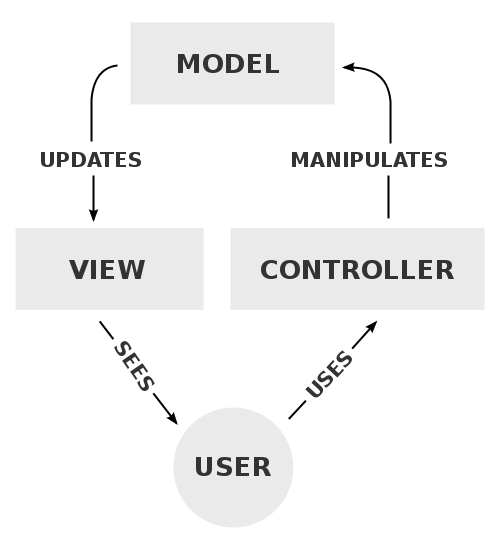
\includegraphics[scale=0.4]{MVC.jpg}
\end{center}
\end{frame}

\begin{frame}
\frametitle{O padrão MVC}
\framesubtitle{A tríade: os três componentes do MVC}
\begin{itemize}
	\item Model: encapsula os dados e a funcionalidade. É independente de representações específicas das saídas de dados e do comportamento da entrada de dados
	\item View: apresenta as informações para o usuário. Os dados apresentados são obtidos do model. Podem haver diversas views para um model
	\item Controller: cada view tem um controller associado à ela. Controllers recebem eventos de entrada, como click de mouse ou leitura de teclado. Tais eventos são então traduzidos em requisições para o model ou para a view. É pelo controller que o usuário interage com o sistema
\end{itemize}
\end{frame}

\begin{frame}
\frametitle{O padrão MVC}
\framesubtitle{Padrões associados}
\begin{itemize}
	\item Observer: mantém as views e os controllers sincronidados com o model
	\item Composite: permite a criação de views compostas, contendo outras views
	\item Strategy: permite a utilização de diferentes controllers para uma mesma view
\end{itemize}
\end{frame}

\begin{frame}
\frametitle{O padrão MVC}
\framesubtitle{Padrões associados - Observer}
	O padrão \textit{Observer} é uma peça chave na implementação original do MVC. Ele é utilizado para que as views e os controllers mantenham-se sincronizados com os models, recebendo mensagens sobre alterações, sem que o model tenha conhecimento das views e dos controllers, mantendo o baixo acoplamento
\end{frame}

\begin{frame}
\frametitle{O padrão MVC}
\framesubtitle{Padrões associados - Observer}
	\begin{center}
		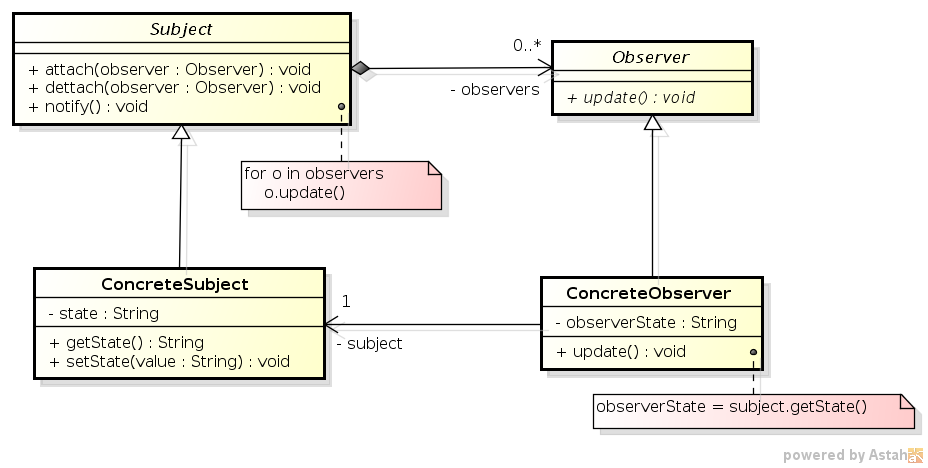
\includegraphics[scale=0.45]{Observer.png}
	\end{center}
\end{frame}

\begin{frame}
\frametitle{O padrão MVC}
\framesubtitle{Padrões associados - Observer}
	\begin{center}
		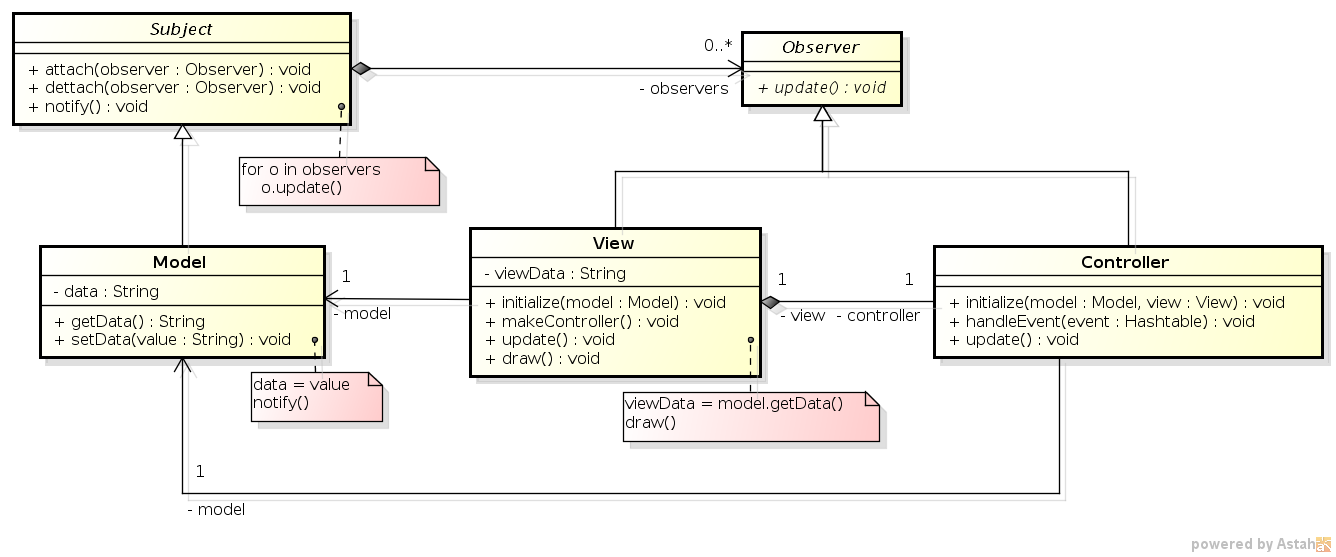
\includegraphics[scale=0.32]{ClassicMVC.png}
	\end{center}
\end{frame}

\begin{frame}
\frametitle{O padrão MVC}
\framesubtitle{Padrões associados - Composite}
	O padrão \textit{Composite} permite a criação de CompositeViews, tendo várias views filhas responsáveis por cada elemento da interface de usuário. Uma tela pode ser implementada como uma CompositeView que possui uma view para um campo texto, outra para um botão, outra para uma caixa de seleção, etc
\end{frame}

\begin{frame}
\frametitle{O padrão MVC}
\framesubtitle{Padrões associados - Strategy}
	O padrão \textit{Strategy} permite a utilização de diferentes modos de entrada e interação do usuário através da escolha de diferentes controllers para uma mesma view. É possível, por exemplo, ter um controller mais focado na interação utilizando o mouse e outro focado na utilização de atalhos do teclado, bastando inicializar um ou outro controler para comportamentos diferentes
\end{frame}

\begin{frame}
\frametitle{Alguns frameworks que usam MVC ou derivados}
\framesubtitle{}
	\textbf{ActionScript 3} - Cairngorm, PureMVC\\
	\textbf{ASP} - ASP Xtreme Evolution, Toika, AJAXED\\
	\textbf{Java} - Apache Struts, Tapestry, VRaptor, Spring MVC, JSF\\
	\textbf{Perl} - Catalyst\\
	\textbf{PHP} - CakePHP, CodeIgniter, LightVC, Symfony\\
	\textbf{Python} - Django\\
	\textbf{Ruby} - Rails\\
	\textbf{Smalltalk} - Smalltalk-80\\
	\textbf{Javascript} (server side) - Sails.js\\
	\textbf{Javascript} (client side) - AngularJs, Backbone.js, Ember.js\\
\end{frame}

\begin{frame}
\frametitle{Alguns frameworks que usam MVC ou derivados}
\framesubtitle{Rails não é MVC puro!}
	Apesar do que se diz por aí, o famoso framework \textit{Rails}, para \textit{Ruby}, não é MVC, ou pelo menos, não o clássico,
	mas sim um modelo derivado deste, chamado \textbf{Model 2}
\end{frame}

\begin{frame}
\frametitle{Alguns frameworks que usam MVC ou derivados}
\framesubtitle{Rails não é MVC puro!}
	No MVC clássico, um model pode notificar as views a respeito das mudanças que aconteceram (a partir do padrão \textit{Observer}). No Rails
	nós não notificamos as views a partir do model, o controller simplesmente passa o dado do model para a view que se encarrega da geração do HTML que
	é posteriormente enviado ao browser, como exibido no esquema abaixo:
	\begin{center}
		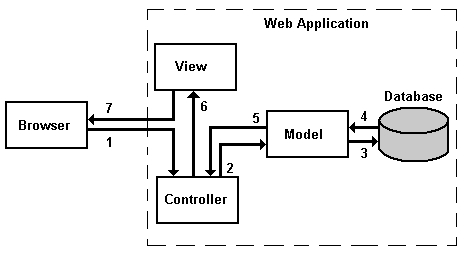
\includegraphics[scale=0.35]{RailsMVC.jpg}
	\end{center}
\end{frame}

\begin{frame}
\frametitle{Alguns padrões similares ao MVC}
\framesubtitle{O Model 2}
	A seguir, um diagrama do \textit{Design Pattern} \textbf{Model 2}, usado no framework \textit{Rails}, mencionado no último slide
	\begin{center}
		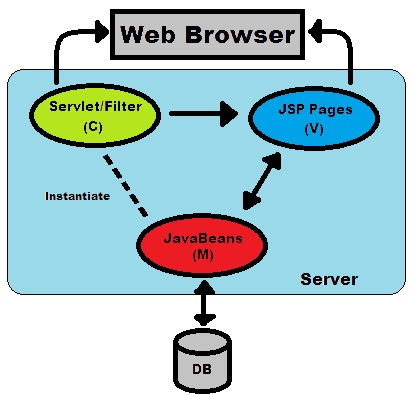
\includegraphics[scale=0.2]{Model2.jpg}
	\end{center}
	As requisições do navegador do cliente são passadas para o controller. Na seqüência, o controller faz o que precisa para obter o conteúdo que deve ser exibido.
	Em seguida, o conteúdo é colocado na requisição, freqüentemente como um JavaBean, e é decidido para qual view o conteúdo será repassado para então, finalmente, esta
	view renderizá-lo
\end{frame}

\begin{frame}
\frametitle{Alguns padrões similares ao MVC}
\framesubtitle{O Hierarchical Model–View–Controller (HMVC)}
	O \textbf{HMVC} é uma variação do MVC, similar a um outro chamado \textit{Presentation–Abstraction–Control (PAC)}, que surgiu como uma tentativa de resposta aos problemas de escalabilidade.
	\begin{center}
		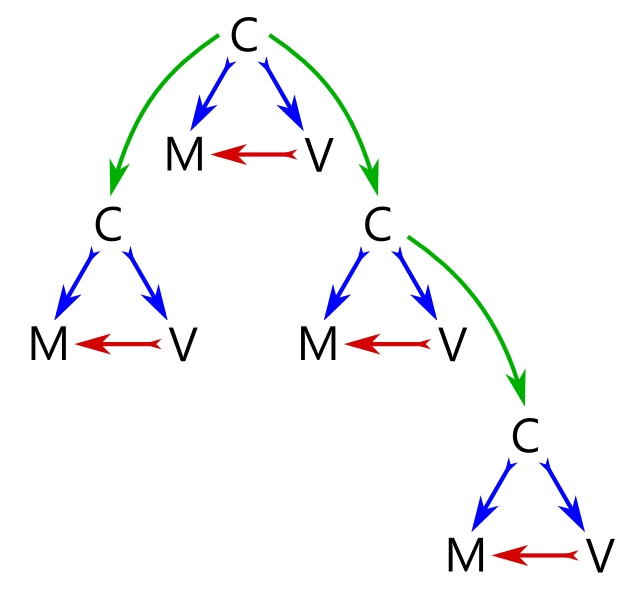
\includegraphics[scale=0.175]{HMVC.jpg}
	\end{center}
	Cada tríade funciona independentemente e uma tríade pode fazer requisição de acesso à outra a partir dos seus controllers.
\end{frame}

\begin{frame}
\frametitle{Alguns padrões similares ao MVC}
\framesubtitle{MVC versus HMVC: algumas diferenças}
	\begin{itemize}
	\item MVC é mais simples.
	\item HMVC é mais escalável.
\end{itemize}
\end{frame}

\begin{frame}
\frametitle{Alguns padrões similares ao MVC}
\framesubtitle{O Movel-View-Adapter (MVA)}
	Uma outra variação do MVC é o \textbf{Model-View-Adapter (MVA)}, mostrado a seguir:
	\begin{center}
		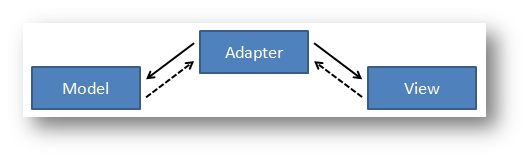
\includegraphics[scale=0.4]{MVA.jpg}
	\end{center}
	Na imagem, as linhas pontilhadas representam comunicação indireta, através do uso do padrão \textit{Observer}, já as demais linhas são relações diretas.
\end{frame}

\begin{frame}
\frametitle{Alguns padrões similares ao MVC}
\framesubtitle{MVC versus MVA: algumas diferenças}
\begin{itemize}
	\item Desacoplamento total do model e da view no MVA.
	\item Toda a dinâmica da aplicação é centralizada no adapter.
\end{itemize}
\end{frame}

\begin{frame}
\frametitle{Alguns padrões similares ao MVC}
\framesubtitle{O Movel-View-Presenter (MVP)}
	Nesta outra variação do MVC, nomeada \textbf{Model-View-Presenter (MVP)}, a View é a responsável por manipular os eventos da interface de usuário, função do controller no MVC tradicional
	\begin{center}
		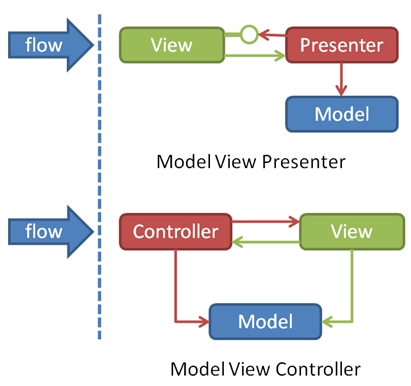
\includegraphics[scale=0.3]{MVP.jpg}
	\end{center}
	O MVP surgiu, dentre outros motivos, com o objetivo de tentar facilitar a realização de testes de unidade automatizados (diferente do MVC tradicional, o presenter
	só interage com a view por meio de uma interface). Aqui, o presenter age sobre o model e a view, atualizando e recuperando dados do model e passando-os já preparados para a view, que apenas deverá exibi-los da maneira esperada.
\end{frame}

\begin{frame}
\frametitle{Alguns padrões similares ao MVC}
\framesubtitle{MVC versus MVP: algumas diferenças}
\begin{itemize}
	\item View está menos amarrada ao model no MVP. Amarrá-los é tarefa do presenter.\\
	\item Mais facilidade para realizar testes de unidade no MVP.\\
	\item Views complexas podem ter múltiplos presenters.
	\item No MVC, a parte lógica deve sempre ficar completamente isolada da view.
	\item Controller é baseado em comportamentos e pode ser compartilhado através das views.
\end{itemize}
\end{frame}

\begin{frame}
\frametitle{Referências}
\begin{itemize}
	\item GAMMA, Erich; HELM, Richard; JOHNSON, Ralph; VLISSIDES, John; \textit{Design Patterns: Elements of Reusable Object-Oriented Software}. 1st Edition. Addison-Wesley. 1995.
	\item SCHMIDT, Douglas C; STAL, Michael; ROHNERT, Hans; BUSCHMANN, Frank; \textit{Pattern-Oriented Software Architecture, Volume 2: Patterns for Concurrent and Networked Objects}. 2nd Edition. John Wiley and Sons. 2000.
	\item FOWLER, Martin; \textit{Patterns of Enterprise Application Architecture}. 1st Edition. Addison-Wesley. 2002.
	\item en.wikipedia.org/
\end{itemize}
\end{frame}

\end{document}
